\documentclass[12pt,letterpaper]{article}
\usepackage{graphicx,textcomp}
\usepackage{natbib}
\usepackage{setspace}
\usepackage{fullpage}
\usepackage{color}
\usepackage[reqno]{amsmath}
\usepackage{amsthm}
\usepackage{fancyvrb}
\usepackage{amssymb,enumerate}
\usepackage[all]{xy}
\usepackage{endnotes}
\usepackage{lscape}
\newtheorem{com}{Comment}
\usepackage{float}
\usepackage{hyperref}
\newtheorem{lem} {Lemma}
\newtheorem{prop}{Proposition}
\newtheorem{thm}{Theorem}
\newtheorem{defn}{Definition}
\newtheorem{cor}{Corollary}
\newtheorem{obs}{Observation}
\usepackage[compact]{titlesec}
\usepackage{dcolumn}
\usepackage{tikz}
\usetikzlibrary{arrows}
\usepackage{multirow}
\usepackage{xcolor}
\newcolumntype{.}{D{.}{.}{-1}}
\newcolumntype{d}[1]{D{.}{.}{#1}}
\definecolor{light-gray}{gray}{0.65}
\usepackage{url}
\usepackage{listings}
\usepackage{color}

\definecolor{codegreen}{rgb}{0,0.6,0}
\definecolor{codegray}{rgb}{0.5,0.5,0.5}
\definecolor{codepurple}{rgb}{0.58,0,0.82}
\definecolor{backcolour}{rgb}{0.95,0.95,0.92}

\lstdefinestyle{mystyle}{
	backgroundcolor=\color{backcolour},   
	commentstyle=\color{codegreen},
	keywordstyle=\color{magenta},
	numberstyle=\tiny\color{codegray},
	stringstyle=\color{codepurple},
	basicstyle=\footnotesize,
	breakatwhitespace=false,         
	breaklines=true,                 
	captionpos=b,                    
	keepspaces=true,                 
	numbers=left,                    
	numbersep=5pt,                  
	showspaces=false,                
	showstringspaces=false,
	showtabs=false,                  
	tabsize=2
}
\lstset{style=mystyle}
\newcommand{\Sref}[1]{Section~\ref{#1}}
\newtheorem{hyp}{Hypothesis}

\title{Problem Set 2}
\date{Due: October 14, 2024}
\author{Applied Stats/Quant Methods 1}

\begin{document}
	\maketitle
	\vspace{-2em} 
	\noindent \textbf{Name: Ombeline Mussat} \\
	\noindent \textbf{Student Number: 24346050} \\
	\vspace{1cm}
	

	\section*{Question 1: Political Science}
		\vspace{.25cm}
	The following table was created using the data from a study run in a major Latin American city.\footnote{Fried, Lagunes, and Venkataramani (2010). ``Corruption and Inequality at the Crossroad: A Multimethod Study of Bribery and Discrimination in Latin America. \textit{Latin American Research Review}. 45 (1): 76-97.} As part of the experimental treatment in the study, one employee of the research team was chosen to make illegal left turns across traffic to draw the attention of the police officers on shift. Two employee drivers were upper class, two were lower class drivers, and the identity of the driver was randomly assigned per encounter. The researchers were interested in whether officers were more or less likely to solicit a bribe from drivers depending on their class (officers use phrases like, ``We can solve this the easy way'' to draw a bribe). The table below shows the resulting data.


\begin{table}[h!]
	\centering
	\begin{tabular}{l | c c c }
		& Not Stopped & Bribe requested & Stopped/given warning \\
		\\[-1.8ex] 
		\hline \\[-1.8ex]
		Upper class & 14 & 6 & 7 \\
		Lower class & 7 & 7 & 1 \\
		\hline
	\end{tabular}
\end{table}

\newpage

\begin{enumerate}
	
	\item [(a)]
	Calculate the $\chi^2$ test statistic by hand/manually (even better if you can do "by hand" in \texttt{R}).\\
	\vspace{0.2cm}
	
	To calculate the $\chi^2$ test statistic, we need to get both the expected and observed frequency for each observation. 
	We can see the observed frequency from the table above (the row count), so we have:
	
	\lstinputlisting[language=R, firstline=6, lastline=11]{/Users/ombelinemussat/Documents/GitHub/StatsI_Fall2024/problemSets/PS02/my_answers/PS02_OM.R}
	
	
	let's first calculate the expected frequency of each observation:
	\[
	f_{\text{expected}} = \frac{\frac{\text{Row Total}}{\text{Grand Total}}}{\text{Column Total}}
	\]
	We can compute all the expected frquencies in R, and then display the results:
	\lstinputlisting[language=R, firstline=13, lastline=24]{/Users/ombelinemussat/Documents/GitHub/StatsI_Fall2024/problemSets/PS02/my_answers/PS02_OM.R}
	 
	 We have the following table:
	 
	 
\begin{table}[h!]
	\centering
	\scriptsize % Reduce font size to scriptsize
	\begin{tabular}{l | c c c | c }
		& Not Stopped & Bribe requested & Stopped/given warning & Total \\
		\\[-1.8ex] 
		\hline \\[-1.8ex]
		Upper class & $f_{\text{observed11}}=14$, $f_{\text{expected11}}=13.5$ 
		& $f_{\text{observed12}}=6$,  $f_{\text{expected12}}=8.36$
		& $f_{\text{observed13}}=7$, $f_{\text{expected13}}=5.14$
		& $27$ \\
		
		Lower class & $f_{\text{observed21}}=7$, $f_{\text{expected21}}=7.5$ 
		& $f_{\text{observed22}}=7$, $f_{\text{expected22}}=4.64$
		& $f_{\text{observed23}}=1$, $f_{\text{expected23}}=2.86$
		& $15$ \\
		\hline
		Total & $21$ & $13$ & $8$ & $42$ \\
	\end{tabular}
\end{table}


\newpage
	 
	 Then, we can calculate the $\chi^2$ test statistic using this formula
	 \[
	 \chi^2 = \sum \frac{(f_{\text{observed}} - f_{\text{expected}})^2}{f_{\text{expected}}}
	 \]
	 
	
	With our calculations of each observed and expected frequencies, we have:
	\[
	\chi^2 = 
	\begin{split}
		\frac{(f_{\text{observed}_{11}} - f_{\text{expected}_{11}})^2}{f_{\text{expected}_{11}}} 
		+ \frac{(f_{\text{observed}_{12}} - f_{\text{expected}_{12}})^2}{f_{\text{expected}_{12}}} 
		+ \frac{(f_{\text{observed}_{13}} - f_{\text{expected}_{13}})^2}{f_{\text{expected}_{13}}} \\
		+ \frac{(f_{\text{observed}_{21}} - f_{\text{expected}_{21}})^2}{f_{\text{expected}_{21}}} 
		+ \frac{(f_{\text{observed}_{22}} - f_{\text{expected}_{22}})^2}{f_{\text{expected}_{22}}} 
		+ \frac{(f_{\text{observed}_{23}} - f_{\text{expected}_{23}})^2}{f_{\text{expected}_{23}}} 
	\end{split}
	\]
	

	 We can compute this equation in R:
	 \lstinputlisting[language=R, firstline=31, lastline=32]{/Users/ombelinemussat/Documents/GitHub/StatsI_Fall2024/problemSets/PS02/my_answers/PS02_OM.R}
	 
	 We get a  $\chi^2$ test statistic of  \(3.8\). 
	
	\vspace{1cm}
	\item [(b)]
	
	Now calculate the p-value from the test statistic you just created (in \texttt{R}).\footnote{Remember frequency should be $>$ 5 for all cells, but let's calculate the p-value here anyway.}  What do you conclude if $\alpha = 0.1$?\\
	
	Let's calculate the p-value from the test statistic we just reated.
	First, we need to compute the degree of freedom.
	\[
	df = (\text{rows} - 1)(\text{columns} - 1)
	\]
	

	
	We have a degree of freedom df = \(2\).
	
		
	We can then calculate the p-value with the following formula:
	\lstinputlisting[language=R, firstline=39, lastline=40]{/Users/ombelinemussat/Documents/GitHub/StatsI_Fall2024/problemSets/PS02/my_answers/PS02_OM.R}

	
	We get a p-value of  \(0.15\). If  \(\alpha = 0.1\), so \( \text{p-value} > \alpha \), we cannot conclude that there is a statistically significant difference in the likelihood of police officers soliciting bribes based on the class of the driver (upper class vs. lower class). Therefore, this suggests that the variables (policers soliciting bribes and social class) may be statistically independent in this context
	
	

	\newpage
	\item [(c)] Calculate the standardized residuals for each cell and put them in the table below.
	\vspace{1cm}
	
	Let's calculate the standardised residuals. The standardised residual tells us how far an observation is from the expectation. 
	First we need to calculate the adjusted residual for each cell (z-score).
	The z-score can be calculated as follows:
	\[
	z = \frac{f_{\text{observed}} - f_{\text{expected}}}{\sqrt{f_{\text{expected}}(1 - \text{row proportion})(1 - \text{column proportion})}}
	\]
	
	
	Let's calculate each of them in R:
	\lstinputlisting[language=R, firstline=48, lastline=59]{/Users/ombelinemussat/Documents/GitHub/StatsI_Fall2024/problemSets/PS02/my_answers/PS02_OM.R}
	
We have the following results:
	
	\begin{table}[h]
		\centering
		\begin{tabular}{l | c c c }
			& Not Stopped & Bribe requested & Stopped/given warning \\
			\\[-1.8ex] 
			\hline \\[-1.8ex]
			Upper Class  & \( z_{11}=0.3220306 \) & \( z_{12}=-1.641957 \) & \( z_{13}=1.523026\) \\
			\\
			Lower Class & \( z_{21}=-0.3220306 \) & \( z_{22}=1.641957 \) & \( z_{23} =-1.523026\) \\
			
		\end{tabular}
	\end{table}
	
	
	\vspace{0.5cm}
	\item [(d)] How might the standardized residuals help you interpret the results?  
	\vspace{0.5cm}
	
	
	These standardised residuals tell us how far away each observed value is from its expectation. A larger (positive or negative) standardised residual indicates that the observed count is much higher (if positive) or lower (if negative) than the expected. For example, \( z_{12} = -1.641957 \) for the Upper Class with a Bribe requested suggests that the Upper Class is less likely than expected to have a bribe requested. On the opposite, \( z_{22} = 1.641957 \) for the Lower Class indicates that they are more likely than expected to have a bribe requested to them. \\
	
	
	With these standardised residuals, we can also conclude our chi-squared test. \\
	We can compare these standardised residuals to a critical value (for example, \( \pm 2 \) for a 95\% confidence interval). If \( \lvert Z^* \rvert \) is bigger than 2, the p-value associated with that residual will be smaller than \( \alpha = 0.05 \). If this is the case, we can reject the null hypothesis. Since we are running a chi-squared test, and testing whether the variables are independent, If \( \lvert Z^* \rvert \) is bigger than 2, it would mean that we have enough evidence to say that those variables are not independent (reject the null hypothesis).\\
	In our example, none of the standardised residuals exceeds this critical value (all the absolute values are below 2), so we would fail to reject the null hypothesis. \\
	Also, if the standardised residual exceeds  \( \pm 3 \), it is an even stronger evidence that the observed count differs significantly from the expected count, suggesting a true association between the variables. Since none of the standardised residuals calculated are above 3 and below -3, we have no strong evidence of an association between the variables. \\
	We can conclude that the differences between the observed and expected counts are not statistically significant, and we do not have enough evidence to conclude that the variables are dependent.
	

	
	
	
\end{enumerate}
\newpage

\section*{Question 2: Economics}
Chattopadhyay and Duflo were interested in whether women promote different policies than men.\footnote{Chattopadhyay and Duflo. (2004). ``Women as Policy Makers: Evidence from a Randomized Policy Experiment in India. \textit{Econometrica}. 72 (5), 1409-1443.} Answering this question with observational data is pretty difficult due to potential confounding problems (e.g. the districts that choose female politicians are likely to systematically differ in other aspects too). Hence, they exploit a randomized policy experiment in India, where since the mid-1990s, $\frac{1}{3}$ of village council heads have been randomly reserved for women. A subset of the data from West Bengal can be found at the following link: \url{https://raw.githubusercontent.com/kosukeimai/qss/master/PREDICTION/women.csv}\\

\noindent Each observation in the data set represents a village and there are two villages associated with one GP (i.e. a level of government is called "GP"). Figure~\ref{fig:women_desc} below shows the names and descriptions of the variables in the dataset. The authors hypothesize that female politicians are more likely to support policies female voters want. Researchers found that more women complain about the quality of drinking water than men. You need to estimate the effect of the reservation policy on the number of new or repaired drinking water facilities in the villages.
\vspace{.5cm}
\begin{figure}[h!]
	\caption{\footnotesize{Names and description of variables from Chattopadhyay and Duflo (2004).}}
	\vspace{.5cm}
	\centering
	\label{fig:women_desc}
	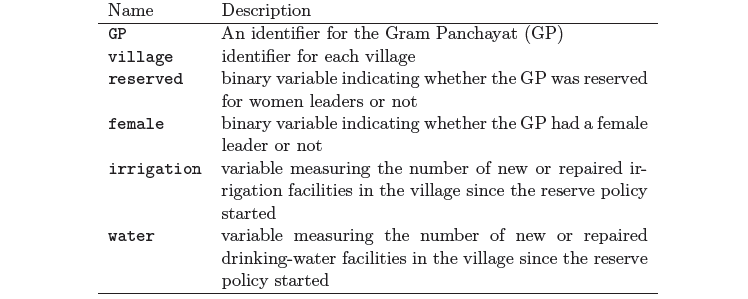
\includegraphics[width=1.1\textwidth]{women_desc.png}
\end{figure}		

\newpage
\begin{enumerate}
	\item [(a)] State a null and alternative (two-tailed) hypothesis. 
	
	We want to find out if there is an effect of the reservation policy on the number of new or repaired drinking water facilities in the villages.
	
	First, we give the assumptions before stating the hypotheses. We have 4 assumptions:\\
	1. The data is generated randomly. \\
	2. The observations are independent. \\
	3. Linearity: The population means of \( Y \) at different values of \( X \) have a straight-line relationship with \( X \): \( \mu_{y|x} = \beta_0 + \beta_1 x \). \\
	4. The errors are normally distributed, with mean 0 and a constant variance:\\ \( \varepsilon_i \sim N(0, \sigma^2) \). \\
	
	Thus we have a null hypothesis:
	\[
	H_0: \beta_{\text{policy}} = 0
	\]
	If the coefficient \( \beta_{\text{policy}} \) in the model equals zero, this would mean that the reservation policy has no effect on the number of new or repaired drinking water facilities. 
	
	The alternative hypothesis would be:
	\[
	H_a: \beta_{\text{policy}} \neq 0
	\]
	
	If the coefficient \( \beta_{\text{policy}} \) in the model does not equal zero, this would mean that the reservation policy does have an effect on the number of new or repaired drinking water facilities.
	
	
	\vspace{1cm}
	\item [(b)] Run a bivariate regression to test this hypothesis in \texttt{R} (include your code!).
	
	Let's run a bivariate regression to test this hypothesis in R, we first have to load the data from github. 
	
	\lstinputlisting[language=R, firstline=78, lastline=80]{/Users/ombelinemussat/Documents/GitHub/StatsI_Fall2024/problemSets/PS02/my_answers/PS02_OM.R}
	
	Then we have to define what our X (explanatory) and Y (response) variables are.
	
	\lstinputlisting[language=R, firstline=82, lastline=83]{/Users/ombelinemussat/Documents/GitHub/StatsI_Fall2024/problemSets/PS02/my_answers/PS02_OM.R}
	
	We can finally run the regression. 

	\lstinputlisting[language=R, firstline=85, lastline=88]{/Users/ombelinemussat/Documents/GitHub/StatsI_Fall2024/problemSets/PS02/my_answers/PS02_OM.R}
	
	\newpage
	We have the results of the regression: 
	
	\begin{verbatim}
		Call:
		lm(formula = Y ~ X, data = data)
		
		Residuals:
		Min      1Q  Median      3Q     Max 
		-23.991 -14.738  -7.865   2.262 316.009 
		
		Coefficients:
		Estimate Std. Error t value Pr(>|t|)    
		(Intercept)   14.738      2.286   6.446 4.22e-10 ***
		X              9.252      3.948   2.344   0.0197 *  
		---
		Signif. codes:  0 ‘***’ 0.001 ‘**’ 0.01 ‘*’ 0.05 ‘.’ 0.1 ‘ ’ 1
		
		Residual standard error: 33.45 on 320 degrees of freedom
		Multiple R-squared:  0.01688,   Adjusted R-squared:  0.0138 
		F-statistic: 5.493 on 1 and 320 DF,  p-value: 0.0197
	\end{verbatim}
	
	
	\vspace{0.5cm}
	\item [(c)] Interpret the coefficient estimate for reservation policy. 
	
	The coefficient estimate for reservation policy is 9.252. It is a positive coefficient, meaning that the reservation policy is associated with more repaired drinking facilities (positive association). \\
	Since \( X \) is a binary variable (whether the GP was reserved for women leaders or not), the intercept, 14.738, represents the estimated number of new or repaired drinking water facilities in villages without the reservation policy (when \( X = 0 \)). When the reservation policy is in effect (when \( X = 1 \)), the total estimated number of new or repaired drinking water facilities is \( 14.738 + 9.252 = 23.99 \). So when the Gram Panchayat (GP) was reserved for women leaders (there was the reservation policy), there was 9.252 more new or repaired drinking-water facilities in the village. \\
	The p-value associated with this coefficient estimate is \( 0.0197 \). This value is less than the significance level (let's say that we use a \( 95\% \) confidence level, \( \alpha = 0.05 \) so \( \text{p-value} < \alpha \)). We can conclude that the effect of the reservation policy on the number of new or repaired drinking-water facilities in the village is statistically significant.



	
\end{enumerate}

\end{document}
